\documentclass[
	12pt,
	oneside,
	a4paper,
	english,
	brazilian,
	sumario=tradicional,
	chapter=TITLE
	]{abntex2}

% Importa toda a "inteligência" e configuração visual da instituição
% ==================================================================
% CONFIGURAÇÕES INSTITUCIONAIS E PACOTES
% Este arquivo consolida todas as configurações visuais, pacotes e 
% macros do Instituto Federal de Sergipe (IFS).
% ==================================================================

% --- Codificação e Tipografia Moderna ---
\usepackage{iftex}
\ifPDFTeX
    \usepackage[utf8]{inputenc}
    \usepackage[T1]{fontenc}
\fi

% --- Fonte acadêmica moderna: Palatino ---
\usepackage{mathpazo} % Tipografia Palatino clássica (inclusa no TeX Live base)
\usepackage[
    activate={true,nocompatibility},
    tracking=true,
    factor=1000,
    stretch=10,
    shrink=10
]{microtype}
\microtypecontext{spacing=nonfrench}

\usepackage{indentfirst}
\usepackage{color}
\usepackage{graphicx}
\usepackage{csquotes}

% --- Matemática e Tabelas ---
\usepackage{amsmath}
\usepackage{booktabs}
\usepackage{tabularx}
\usepackage{multirow}
\usepackage{array}
\usepackage{longtable}
\usepackage{siunitx}

% Configuração nativa do memoir para legendas ABNT (evita usar o pacote caption que conflita)
\captionnamefont{\small\bfseries}
\captiontitlefont{\small}
\captiondelim{ -- } % Padrão ABNT (travessão separando label do texto)

% --- Código-fonte ---
\usepackage{listings}
\usepackage{xcolor}
\usepackage{courier} % Fonte monospace padrão de alta compatibilidade
\renewcommand{\lstlistingname}{Código}
\definecolor{codeBackground}{HTML}{F8F9FA}
\definecolor{codeFrame}{HTML}{DEE2E6}
\definecolor{codeKeyword}{HTML}{0550AE}
\definecolor{codeString}{HTML}{0A3069}
\definecolor{codeComment}{HTML}{6E7781}
\definecolor{codeNumber}{HTML}{953800}
\lstset{
    backgroundcolor  = \color{codeBackground},
    basicstyle       = \ttfamily\small,
    keywordstyle     = \color{codeKeyword}\bfseries,
    stringstyle      = \color{codeString},
    commentstyle     = \color{codeComment}\itshape,
    numberstyle      = \tiny\color{codeNumber},
    numbers          = left,
    keepspaces       = true,
    columns          = fullflexible,
    upquote          = true,
    numbersep        = 8pt,
    frame            = single,
    rulecolor        = \color{codeFrame},
    framesep         = 6pt,
    xleftmargin      = 16pt,
    framexleftmargin = 16pt,
    breaklines       = true,
    breakatwhitespace= true,
    showstringspaces = false,
    tabsize          = 4,
    captionpos       = t,
    aboveskip        = 12pt,
    belowskip        = 12pt,
    literate         = {á}{{\'a}}1 {é}{{\'e}}1 {í}{{\'i}}1 {ó}{{\'o}}1
                       {ú}{{\'u}}1 {ã}{{\~a}}1 {õ}{{\~o}}1
                       {ç}{{\c{c}}}1 {Ç}{{\c{C}}}1
                       {ê}{{\^e}}1 {â}{{\^a}}1
}

% --- Listas ---
\usepackage{enumitem}
\setlist{
    topsep     = 0pt,
    itemsep    = 0pt,
    parsep     = 4pt,
    leftmargin = \parindent
}
\setlist[enumerate]{label=\arabic*.}
\setlist[itemize]{label=\textbullet}

% --- Referências e Hiperlinks ---
\usepackage[style=abnt, justify, maxbibnames=99, sorting=nty]{biblatex}
\setlength{\bibitemsep}{\baselineskip} % Espaçamento de 1 linha entre referências distintas (ABNT NBR 6023)
\addbibresource{referencias.bib}

\usepackage{xurl}
\urlstyle{same}
\usepackage{hyperref}
\hypersetup{
    colorlinks     = true,
    linkcolor      = black,
    citecolor      = black,
    filecolor      = black,
    urlcolor       = black,
    bookmarksdepth = 4
}

% --- Margens e Espaçamentos (ABNT) ---
\setlrmarginsandblock{3cm}{2cm}{*}
\setulmarginsandblock{3cm}{2cm}{*}
\checkandfixthelayout

\OnehalfSpacing
\setlength{\parindent}{1.25cm}
\setlength{\ABNTEXcitacaorecuo}{4cm}

\widowpenalty=10000
\clubpenalty=10000

% --- Estilização Acadêmica Sóbria ---
\renewcommand{\ABNTEXchapterfont}{\normalfont\bfseries}
\renewcommand{\ABNTEXchapterfontsize}{\normalsize} % NBR 14724 exige fonte tamanho 12 uniforme
\renewcommand{\ABNTEXsectionfont}{\normalfont\bfseries}
\renewcommand{\ABNTEXsectionfontsize}{\normalsize}
\renewcommand{\ABNTEXsubsectionfont}{\normalfont\bfseries}
\renewcommand{\ABNTEXsubsectionfontsize}{\normalsize}
\setboolean{ABNTEXuppersection}{false} % Apenas capítulos ficam em caixa alta, seções secundárias em caixa baixa

% Nomes de elementos pré e pós-textuais em maiúsculas (ABNT NBR 14724)
\addto\captionsbrazilian{
    \renewcommand{\bibname}{REFERÊNCIAS}
    \renewcommand{\contentsname}{SUMÁRIO}
    \renewcommand{\listfigurename}{LISTA DE FIGURAS}
    \renewcommand{\listtablename}{LISTA DE TABELAS}
}

\setlength{\beforechapskip}{18pt}
\setlength{\afterchapskip}{1.5\baselineskip}
\chapterstyle{abnt}

\renewcommand{\cftdot}{.}
\renewcommand{\cftdotsep}{3}
\setlength{\cftbeforechapterskip}{0.3em}

% ==================================================================
% MACROS DE IMPRESSÃO (CAPA E FOLHA DE ROSTO IFS)
% ==================================================================

\renewcommand{\imprimircapa}{%
  \begin{capa}%
    \center\bfseries % Todos os elementos da capa em negrito e centralizados (padrão institucional)
    \OnehalfSpacing
    
    
\includegraphics[width=3.2cm]{logo_ifs.png}\par
    \vspace{0.5cm}
    
    {\normalsize\MakeUppercase{\imprimirinstituicao}\par}
    
    \vspace{3.0cm}
    
    {\normalsize\MakeUppercase{\imprimirautor}\par}
    
    \vspace{3.0cm}
    
    {\normalsize\MakeUppercase{\imprimirtitulo}\par}
    
    \vfill
    
    {\normalsize\MakeUppercase{\imprimirlocal}\par}
    {\normalsize\imprimirdata\par}
  \end{capa}
}

\makeatletter
\renewcommand{\imprimirfolhaderosto}{%
  \begin{folhaderosto}
    \center
    \OnehalfSpacing
    
    \vspace*{2cm}
    
    {\normalsize\MakeUppercase{\imprimirautor}\par}
    
    \vspace{4.0cm}
    
    {\normalsize\bfseries\MakeUppercase{\imprimirtitulo}\par}
    
    \vspace{2.0cm}
    
    \begin{flushright}
    \begin{minipage}{8cm}
        \SingleSpacing
        \normalsize
        \imprimirpreambulo\par
        \vspace{0.5cm}
        Orientador: \imprimirorientador
    \end{minipage}
    \end{flushright}
    
    \vfill
    
    {\normalsize\MakeUppercase{\imprimirlocal}\par}
    {\normalsize\imprimirdata\par}
  \end{folhaderosto}
}
\makeatother

% ==================================================================
% FIM DAS CONFIGURAÇÕES
% ==================================================================


% ==========================================
% DADOS DO TRABALHO E DO AUTOR
% ==========================================
% Os dados pessoais, título e orientador ficam isolados em metadados.tex
% para evitar conflitos de versão ao atualizar o template.
\IfFileExists{metadados.tex}{% ==============================================================================
% DADOS DO TRABALHO E DO AUTOR (Área do Aluno)
% ==============================================================================
% Preencha com as informações oficiais do seu Trabalho de Conclusão de Curso (TCC).
% 
% DICA DE ATUALIZAÇÃO:
% Este arquivo é isolado do restante do template para que você possa atualizar
% as configurações do LaTeX e scripts no futuro (via 'make update') sem que seus
% dados pessoais ou título do trabalho entrem em conflito de versão!
% ==============================================================================

\titulo{Avaliação Experimental de Arquiteturas Baseadas em RAG e MCP}
\autor{José Gustavo Correia Nascimento}
\local{Lagarto -- SE}
\data{2026}
\instituicao{%
    Instituto Federal de Educação, Ciência e Tecnologia de Sergipe\par
    Campus Lagarto\par
    Bacharelado em Sistemas de Informação
}
\tipotrabalho{Trabalho de Conclusão de Curso}
\preambulo{Trabalho de Conclusão de Curso apresentado ao curso de Bacharelado em Sistemas de Informação do Instituto Federal de Educação, Ciência e Tecnologia de Sergipe, \textit{Campus} Lagarto, como requisito parcial para obtenção do grau de Bacharel em Sistemas de Informação.}
\orientador{Prof. Diego Armando}
% \coorientador{Prof. Nome do Coorientador} % (Descomente se houver)
}{}

\begin{document}

\frenchspacing

% ------------------------------------------------------------------
% ELEMENTOS PRÉ-TEXTUAIS
% ------------------------------------------------------------------
\imprimircapa
\imprimirfolhaderosto

% Colocar quando precisa realmente % ==========================================
% [BLOCO] DEDICATÓRIA
% ==========================================
\begin{dedicatoria}
   \vspace*{\fill}
   \begin{flushright}
   \noindent
   % [AGENT: INSERIR TEXTO DA DEDICATÓRIA AQUI]
   Este trabalho é dedicado aos meus pais, amigos e a todos 
   que contribuíram direta ou indiretamente para a minha formação.
   \end{flushright}
\end{dedicatoria}

% ==========================================
% [BLOCO] AGRADECIMENTOS
% ==========================================
\begin{agradecimentos}
% [AGENT: INSERIR TEXTO DOS AGRADECIMENTOS AQUI]
Agradeço primeiramente a Deus.
Aos meus familiares pelo apoio incondicional.
Ao meu orientador pela paciência e direcionamento durante toda a pesquisa.
\end{agradecimentos}

% ==========================================
% [BLOCO] EPÍGRAFE
% ==========================================
\begin{epigrafe}
    \vspace*{\fill}
    \begin{flushright}
    % [AGENT: INSERIR TEXTO DA EPÍGRAFE AQUI]
    \textit{``A imaginação é mais importante que o conhecimento.\\
    O conhecimento é limitado. A imaginação circunda o mundo.''\\
    (Albert Einstein)}
    \end{flushright}
\end{epigrafe}

% ==========================================
% [BLOCO] RESUMO EM PORTUGUÊS
% ==========================================
\begin{resumo}
    \noindent
    % [AGENT: INSERIR TEXTO DO RESUMO AQUI]
    O resumo deve ressaltar o objetivo, o método, os resultados e as conclusões do documento. A ordem e a extensão destes itens dependem do tipo de resumo (informativo ou indicativo) e do tratamento que cada item recebe no documento original.
    
    \vspace{\onelineskip}
    \noindent
    \textbf{Palavras-chave}: % [AGENT: INSERIR PALAVRAS-CHAVE AQUI SEPARADAS POR PONTO]
    TCC. LaTeX. Sistemas de Informação. IFS.
\end{resumo}

% ==========================================
% [BLOCO] ABSTRACT EM INGLÊS
% ==========================================
\begin{resumo}[Abstract]
    \begin{otherlanguage*}{english}
        \noindent
        % [AGENT: INSERIR TEXTO DO ABSTRACT AQUI]
        The abstract should highlight the objective, method, results, and conclusions of the document.
        
        \vspace{\onelineskip}
        \noindent
        \textbf{Keywords}: % [AGENT: INSERIR KEYWORDS AQUI SEPARADAS POR PONTO]
        Undergraduate Thesis. LaTeX. Information Systems. IFS.
    \end{otherlanguage*}
\end{resumo}


% ------------------------------------------------------------------
% SUMÁRIO
% ------------------------------------------------------------------
\pdfbookmark[0]{\contentsname}{toc}
\tableofcontents*
\cleardoublepage

% ------------------------------------------------------------------
% ELEMENTOS TEXTUAIS (CAPÍTULOS)
% ------------------------------------------------------------------
\textual

\chapter{Introdução}
% [AGENT: INSERIR TEXTO DA INTRODUÇÃO AQUI]
% Dica: Apresente o contexto, a problematização, a justificativa e os objetivos (geral e específicos).

\section{Contextualização}
\label{sec:contextualizacao}

Este é o primeiro capítulo do seu Trabalho de Conclusão de Curso. Para demonstrar a integração de referências, este parágrafo contém uma citação de artigo acadêmico \cite{exemplo2026} e uma citação de página web \cite{devcontainer}. Lorem ipsum dolor sit amet, consectetur adipiscing elit. Sed vitae sollicitudin nibh, congue fringilla risus. Praesent viverra nisl augue, quis malesuada nibh pharetra id. Sed nec augue pellentesque, imperdiet quam sit amet, dapibus justo. Nunc purus velit, cursus id lorem et, fringilla molestie ante. Vestibulum nec feugiat risus. Etiam condimentum lectus ut enim scelerisque, eget blandit magna vestibulum. Integer tellus tortor, faucibus id posuere id, condimentum ac risus. Ut commodo ut nisl ut placerat. Nulla nec molestie nibh. Cras rhoncus nec turpis sed laoreet.

Vestibulum ante ipsum primis in faucibus orci luctus et ultrices posuere cubilia curae; Phasellus commodo volutpat scelerisque. Cras eget arcu at felis finibus mollis. Vestibulum consectetur rutrum quam eget sagittis. Quisque pellentesque placerat purus, vitae blandit lectus placerat ac. Aliquam ac mauris id orci vehicula ullamcorper. Nunc eu dictum erat, id convallis velit. Proin id orci nibh. Ut fermentum convallis tortor ac interdum. Praesent in mauris ante. Maecenas elit nulla, vehicula eget enim vitae, bibendum accumsan mauris. Vestibulum libero diam, faucibus non nisi rutrum, ultricies suscipit dui.

Proin finibus velit sem, et feugiat est laoreet sit amet. Proin vel mattis felis, id finibus turpis. Etiam sagittis, leo non bibendum fermentum, eros lacus cursus leo, non aliquet odio erat tincidunt purus. Aliquam erat volutpat. Aenean tincidunt orci risus, ac porttitor justo gravida ac. Morbi nec accumsan justo. Nam suscipit quam porttitor, finibus sapien in, semper enim. Aenean vitae dignissim lectus. Curabitur vel arcu sed sapien hendrerit fringilla sit amet a orci. Ut nibh massa, finibus ac ullamcorper sit amet, pharetra at mi. Maecenas sagittis lacus ante, eget malesuada risus facilisis sit amet. Fusce id augue et elit accumsan feugiat. Praesent sit amet nibh tempus, laoreet metus nec, pulvinar nisi.

Pellentesque eu purus nulla. Fusce tincidunt euismod elit, id malesuada nisl venenatis eu. Phasellus a finibus nisl, vitae maximus nibh. Donec nibh nunc, elementum ut efficitur malesuada, consectetur vitae enim. Proin erat augue, scelerisque id blandit eget, faucibus non diam. Vestibulum orci nunc, sodales eget eros quis, cursus tincidunt urna. Curabitur id diam velit.

Mauris aliquet hendrerit lacinia. Etiam euismod convallis tortor, sed pharetra dui condimentum nec. Praesent ac diam mollis, dapibus risus sed, consequat ex. Praesent viverra metus in lacus dictum, non mattis arcu rutrum. Integer aliquam dui suscipit mauris vulputate, laoreet facilisis magna iaculis. Vestibulum non odio in lectus fringilla suscipit. Sed in volutpat est. Morbi in nulla nisi. Mauris eget iaculis nisi. Donec viverra fermentum orci.

Fusce vestibulum blandit dolor, vitae iaculis ipsum pellentesque nec. Integer ultrices ante sit amet pretium aliquet. Duis vitae molestie nisl. Ut sit amet eleifend urna, venenatis tincidunt ligula. Integer vitae metus quam. Mauris mattis velit luctus nisl volutpat, ut blandit massa feugiat. Phasellus quis urna consequat, dapibus nunc a, bibendum dolor. Sed at odio neque. Duis malesuada, mauris efficitur fringilla egestas, ex augue consectetur velit, id dictum odio leo vitae ipsum. Mauris sit amet velit congue, sodales magna sed, blandit libero. Lorem ipsum dolor sit amet, consectetur adipiscing elit. Fusce faucibus nisi ac nibh malesuada dignissim. Nullam sed nisi sit amet eros consequat porttitor ac sit amet risus. Curabitur ac consectetur quam. Sed luctus venenatis turpis, non blandit elit. Phasellus ultrices mattis viverra.

\section{Problema de Pesquisa}
\label{sec:problema}
% ------------------------------------------------------------------

Lorem ipsum dolor sit amet, consectetur adipiscing elit. Sed do eiusmod 
tempor incididunt ut labore et dolore magna aliqua. Ut enim ad minim 
veniam, quis nostrud exercitation ullamco laboris nisi ut aliquip ex ea 
commodo consequat \textit{Campus} Lorem?

% ------------------------------------------------------------------
\section{Hipótese}
\label{sec:hipotese}
% ------------------------------------------------------------------

Duis aute irure dolor in reprehenderit in voluptate velit esse cillum 
dolore eu fugiat nulla pariatur. Excepteur sint occaecat cupidatat non 
proident, sunt in culpa qui officia deserunt mollit anim id est laborum.
Curabitur pretium tincidunt lacus. Nulla gravida orci a odio. Nullam 
varius, turpis et commodo pharetra, est eros bibendum elit, nec luctus 
magna felis sollicitudin mauris.

% ------------------------------------------------------------------
\section{Objetivos}
\label{sec:objetivos}
% ------------------------------------------------------------------

\subsection{Objetivo Geral}

Sed ut perspiciatis unde omnis iste natus error sit voluptatem accusantium 
doloremque laudantium, totam rem aperiam, eaque ipsa quae ab illo inventore 
veritatis et quasi architecto beatae vitae dicta sunt explicabo.

\subsection{Objetivos Específicos}

\begin{enumerate}
    \item \textbf{Implementar} lorem ipsum dolor sit amet, consectetur 
    adipiscing elit, sed do eiusmod tempor incididunt.

    \item \textbf{Validar} ut labore et dolore magna aliqua. Ut enim ad 
    minim veniam, quis nostrud exercitation ullamco.

    \item \textbf{Modelar} laboris nisi ut aliquip ex ea commodo 
    consequat (\textit{Tool Descriptions}) duis aute irure dolor in 
    reprehenderit in voluptate.

    \item \textbf{Levantar} velit esse cillum dolore eu fugiat nulla 
    pariatur \textit{Campus} Lorem.

    \item \textbf{Elaborar} excepteur sint occaecat cupidatat non 
    proident (\textit{dataset}) sunt in culpa qui officia deserunt 
    mollit anim id est laborum.

    \item \textbf{Avaliar e comparar} sed ut perspiciatis unde omnis 
    iste natus error sit voluptatem accusantium doloremque laudantium, 
    totam rem aperiam.

    \item \textbf{Analisar} eaque ipsa quae ab illo inventore veritatis 
    et quasi architecto beatae vitae dicta sunt explicabo.
\end{enumerate}

% ------------------------------------------------------------------
\section{Justificativa}
\label{sec:justificativa}
% ------------------------------------------------------------------

Nemo enim ipsam voluptatem quia voluptas sit aspernatur aut odit aut 
fugit, sed quia consequuntur magni dolores eos qui ratione voluptatem 
sequi nesciunt. Neque porro quisquam est, qui dolorem ipsum quia dolor 
sit amet, consectetur, adipisci velit. Sed quia non 
numquam eius modi tempora incidunt ut labore et dolore magnam aliquam 
quaerat voluptatem. Ut enim ad minima veniam, quis nostrum exercitationem 
ullam corporis suscipit laboriosam, nisi ut aliquid ex ea commodi 
consequatur. Quis autem vel eum iure reprehenderit qui in ea voluptate 
velit esse quam nihil molestiae consequatur.

At vero eos et accusamus et iusto odio dignissimos ducimus qui blanditiis 
praesentium voluptatum deleniti atque corrupti quos dolores et quas 
molestias excepturi sint occaecati cupiditate non provident. Similique 
sunt in culpa qui officia deserunt mollitia animi \textit{Campus} Lorem, 
id est laborum et dolorum fuga. Et harum quidem rerum facilis est et 
expedita distinctio. Nam libero tempore, cum soluta nobis est eligendi.
\chapter{Referencial Teórico}
% [AGENT: INSERIR TEXTO DO REFERENCIAL TEÓRICO AQUI]
% Dica: Cite trabalhos relacionados e os conceitos teóricos que sustentam sua pesquisa.

Aqui entra a fundamentação teórica.

\chapter{Metodologia}
% [AGENT: INSERIR TEXTO DA METODOLOGIA AQUI]
% Dica: Descreva o tipo de pesquisa, os instrumentos de coleta de dados e os métodos de análise.

Apresentação da metodologia do trabalho e procedimentos adotados na pesquisa. Como representação visual dos módulos do sistema, a \autoref{fig:metodologia-exemplo} descreve a arquitetura proposta.

\begin{figure}[htbp]
    \centering
    \caption{Visão Geral da Metodologia e Arquitetura Proposta}
    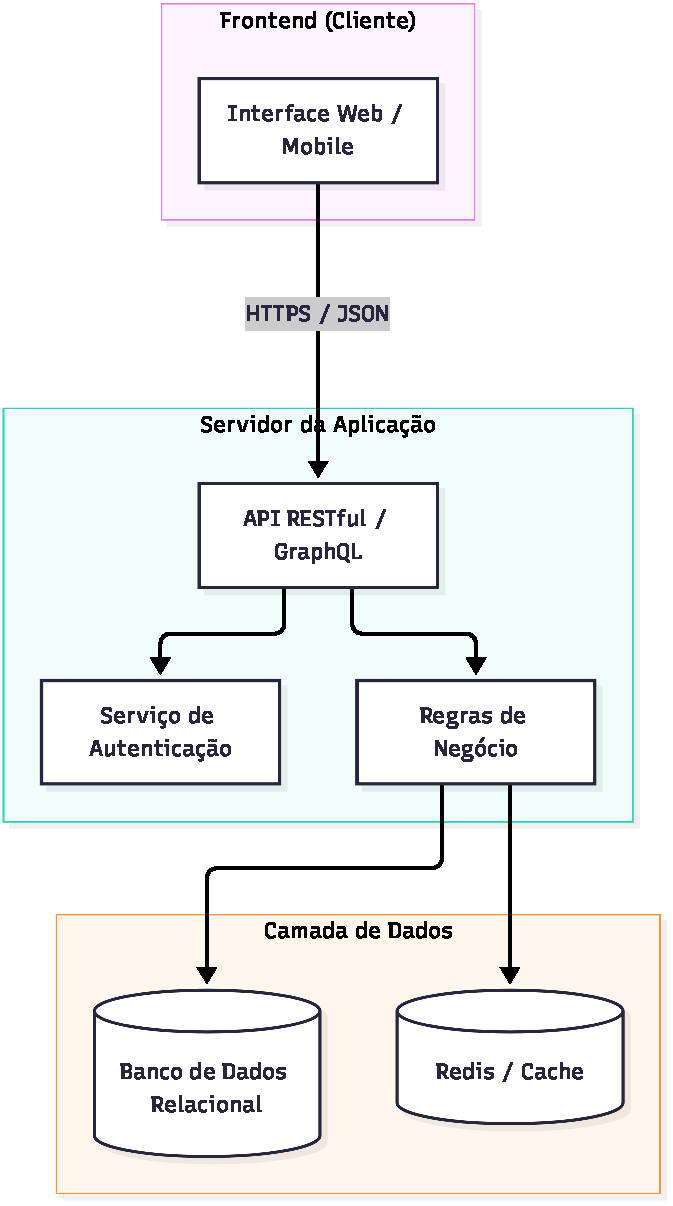
\includegraphics[width=0.85\textwidth,height=0.45\textheight,keepaspectratio]{figuras/exemplo-diagrama.pdf}
    \fonte{Elaborado pelo autor (\the\year).}
    \label{fig:metodologia-exemplo}
\end{figure}

\chapter{Resultados e Discussão}
% [AGENT: INSERIR TEXTO DOS RESULTADOS AQUI]
% Dica: Apresente os dados coletados e discuta-os à luz do referencial teórico.

Análise dos resultados.

\chapter{Conclusão}
% [AGENT: INSERIR TEXTO DA CONCLUSÃO AQUI]
% Dica: Retome os objetivos, apresente as conclusões finais e sugira trabalhos futuros.

Considerações finais do trabalho.


% ------------------------------------------------------------------
% ELEMENTOS PÓS-TEXTUAIS
% ------------------------------------------------------------------
\postextual

\SingleSpacing
\printbibliography[heading=bibintoc]

% ------------------------------------------------------------------
% APÊNDICES (Documentos elaborados pelo próprio autor)
% ------------------------------------------------------------------
\begin{apendicesenv}
    \partapendices
    \chapter{Roteiro de Entrevista Semiestruturada}
\label{apendice:roteiro-entrevista}

Este apêndice apresenta o roteiro de entrevista semiestruturada elaborado pelo autor como instrumento de coleta de dados qualitativos para a avaliação da solução proposta.

\section{Objetivo da Coleta}

Mapear a percepção dos participantes a respeito da usabilidade, desempenho e aderência da arquitetura implementada no contexto de processos acadêmicos e organizacionais.

\section{Blocos de Questões}

\subsection{Bloco 1: Perfil e Experiência do Participante}
\begin{enumerate}
    \item Há quanto tempo você atua na área de Tecnologia da Informação ou desenvolvimento de software?
    \item Qual o seu nível de familiaridade prévio com ferramentas baseadas em Inteligência Artificial generativa?
\end{enumerate}

\subsection{Bloco 2: Avaliação da Arquitetura e Usabilidade}
\begin{enumerate}
    \item Como você avalia a clareza e a responsividade da integração apresentada?
    \item Quais foram os principais desafios ou pontos de atrito identificados durante a execução das tarefas?
    \item Em uma escala de 1 a 5, quão intuitivo foi o fluxo de trabalho automatizado em comparação aos métodos manuais?
\end{enumerate}

\subsection{Bloco 3: Considerações Finais e Sugestões}
\begin{enumerate}
    \item Que funcionalidades ou melhorias adicionais você considera essenciais para futuras iterações deste projeto?
\end{enumerate}

\end{apendicesenv}

% ------------------------------------------------------------------
% ANEXOS (Documentos de terceiros não elaborados pelo autor)
% ------------------------------------------------------------------
\begin{anexosenv}
    \partanexos
    \chapter{Documento de Regulamentação Institucional}
\label{anexo:documento-institucional}

Este anexo reproduz diretrizes normativas ou especificações técnicas externas (não elaboradas pelo autor) que serviram como embasamento regulatório para o desenvolvimento deste Trabalho de Conclusão de Curso.

\section{Identificação da Fonte Reguladora}

\begin{itemize}
    \item \textbf{Órgão Emissor:} Ministério da Educação / Instituto Federal de Educação, Ciência e Tecnologia de Sergipe (IFS).
    \item \textbf{Finalidade:} Critérios de avaliação, prazos regimentais e diretrizes para entrega de Trabalhos de Graduação em Sistemas de Informação.
\end{itemize}

\section{Síntese dos Critérios de Conformidade}

Os procedimentos metodológicos e a infraestrutura implementada observaram as diretrizes de integridade acadêmica, segurança de dados e reprodutibilidade científica estabelecidas pelas normas institucionais vigentes.

\end{anexosenv}

\end{document}
